\documentclass{article}

\usepackage{hyperref}
\usepackage{url}
\usepackage{amsmath}
\usepackage{amsfonts}
\usepackage{latexsym}
\usepackage{graphicx}
%\usepackage{float}
\usepackage[noend]{algorithm2e}

\newcommand{\comment}[1]{}
\newcommand{\field}[1]{\mathbb{#1}} % requires amsfonts
\newcommand{\pd}[2]{\frac{\partial#1}{\partial#2}}

\title{Lock-Free versus Lock based queue/stack data structures}

\author{Fernando Cavalcanti Jeronymo}

\begin{document}

\maketitle

\begin{abstract}
Most implementations of stacks/queues were originally designed for single-threaded processors. With the advent of multi-threaded applications and symmetric multiprocessors those structures can only function by serializing producer/consumer access through a barrier such as lock, mutex, semaphore. Lock-free data structures provide significant performance improvements by allowing multiple producers/consumers to work in parallel without blocking their access to data structures. In this paper, the performance and behavior of lock-free structures are compared against their locked counter parts. Empirical results indicate the inefficiency of lock based structures, such as mutexes, when compared against lock-free implementations, where multi-threaded approaches are computationally slower than single-threaded implementations.
\end{abstract}

\section{Introduction}

Efficient data structures are necessary when considering the ever increasing usage of multi-core and multi-processor systems. The greatest issue in these concurrent environments is to ensure the consistency of shared resources. The usual method for this is mutual exclusion, where the shared resource is locked to a certain process and other concurrent processes must wait to access the resource, \textit{i.e.} causing blocking. However, this degrades the system's performance \cite{Silberschatz08}, and the mutual exclusion process is prone to long delays, convoying, deadlocks, priority inversion and starvation \cite{Sundell08, Gao07}.

Seeking to avoid these problems, researchers have proposed non-blocking algorithms for shared resources \cite{Herlihy91}, commonly known as lock-free algorithms when there is a guaranteed system-wide progress. Lock-free algorithms guarantee threads will never be blocked waiting for another thread to free the resource as it is done with mutual exclusion. Instead, using memory barriers and atomic operations, such as Compare-And-Swap (CAS), they guarantee that only one thread will succeed in going through the critical section and atomically updating resources so that processing time is never wasted while the thread does nothing. The most widely used lock-free algorithm is believed \cite{Lindsay08} to be Michael and Scott's queue algorithm \cite{Michael98}.

In this paper, the performance and behavior of lock-free structures are compared against their locked counter parts, on multi-threaded and single-threaded approaches. Two different systems, one a Linux Server and the other Windows 7, are utilized for analysis of empirical results.

The rest of this paper is organized as follows. Section \ref{sec:lockfree} describes the basics of non-blocking algorithms and lock-free conditions, as well as the pseudocode for single-threaded and multi-threaded queue/stack data structures. Section \ref{sec:results} presents the results of enqueuing and dequeuing 2,000,000 items with single-threaded, lock-free and mutex queue approaches. Finally, in section \ref{sec:conclusion}, a discussion is provided on the empirical results and future work is described.

\section{Lock-Free Queue/Stack Structures}
\label{sec:lockfree}

Queues (First In First Out - FIFO) and Stacks (Last In First Out - LIFO) are very similar data structures. Their similarity and simplicity, compared to more complex data structures such as a map or a hash-table, makes them the perfect choice to be enhanced to use Lock Free Algorithms instead of their mutex based counter-parts. This paper shows the performance gains that can be achieved by using simple lock-free algorithms when running in a concurrent environment. Note that even in a single-CPU architecture a lock free design is desirable when using multiple threads.

\subsection{Defining Lock Free}

A Lock Free approach to algorithm design requires deep understanding about the data structure that is being enhanced as well as what exactly defines a Lock Free algorithm. In lock-free design, one makes use of a memory barrier, usually provided by the Operating System or the Hardware, which guarantees that a thread will never stop its execution, as opposed to a locked approach where mutual exclusion 'mutexes' are used to synchronize critical sections in the code.

In Linux this atomic operation is usually defined as CAS and in gcc compiler both operations are provided as follows:\
\paragraph{CAS}
This builtin atomically compares the data pointed to by 'ptr' against oldval and if equal, meaning it hasn't changed yet, it substitutes it with newval and returns True. Returns False otherwise: \,

	''bool \_sync\_bool\_compare\_and\_swap(type *ptr, type oldval, type newval);''
\paragraph{Memory Barrier}
This builtin issues a full memory barrier: ''\_sync\_synchronize();'' \,

These two operations shall be used as needed to enhance the locked algorithms described later on.

\subsection{Single-Threaded Queue}

As a reference, we first implement a straighforward queue algorithm and run it in a single-thread application. This step will show us how much contention and extra operations, lock/unlock or the memory barrier, will add to the overall cost. Although it would seem that when running the same algorithm in multiple threads would halve the total running time, we will see later that this is counterintuitive and instead the context switching and lock contention, even in the lock free queue, add to the total cost instead of taking from it.

\begin{algorithm}[htp]
\DontPrintSemicolon
\SetKwData{DataPointer}{DataPointer}
\SetKwFunction{Enqueue}{Enqueue}
\SetKwFunction{Dequeue}{Dequeue}
\KwIn{N Data pointer(s)}
\KwOut{The enqueued data pointer}
\For{$i\leftarrow 1$ \KwTo $N$}{
\Enqueue($i$)\;
}
\While{Queue is not empty}{
\DataPointer$\leftarrow$ \Dequeue()\;
}
\caption{Enqueuing/Dequeuing on a single-thread}
\label{alg:mine}
\end{algorithm}

\subsection{Queue Protected with a Mutex}
The Queue is now enhanced with regular pthread\_mutexes so as to protect the critical section, mainly, the queue data structure head, tail and diviser pointers. Then 2 threads are created: A Producer and a Consumer. The data being transferred between threads is a pointer which will have it's size variable, 32-bits or 64-bits depending on which CPU the program is being run on.

The data structure used is a simple c++ std::queue.

\begin{algorithm}[htp]
\BlankLine
\emph{Producer Thread}\;
\caption{Enqueuing with mutexes}
\begin{procedure}[H]
\DontPrintSemicolon
\SetKwFunction{Enqueue}{Enqueue}
\SetKwFunction{Lock}{Lock}
\SetKwFunction{Unlock}{Unlock}
\SetKwData{mutex}{mutex}
\For{$i\leftarrow 1$ \KwTo $N$}{
\Lock(\mutex)\;
\Enqueue($i$)\;
\Unlock(\mutex)\;
}
\label{alg:enq1}
\end{procedure}

\BlankLine
\emph{Consumer Thread}\;
\caption{Dequeuing with mutexes}
\begin{procedure}[H]
\DontPrintSemicolon
\SetKwFunction{Dequeue}{Dequeue}
\SetKwData{DataPointer}{DataPointer}
\SetKwFunction{Lock}{Lock}
\SetKwFunction{Unlock}{Unlock}
\SetKwData{mutex}{mutex}
\While{Queue is not empty}{
\Lock(\mutex)\;
\DataPointer$\leftarrow$ \Dequeue()\;
\Unlock(\mutex)\;
}
\label{alg:deq1}
\end{procedure}

\end{algorithm}

\subsection{Lock Free Queue}

Now we change the Queue to make use of the memory barrier and CAS idioms. There is no need to protect the critical section per-se because each thread cares only about it's own variable, ``first'' for Producer, ``last'' for Consumer and ``divider'' shared between both, while the ``divider`` varible is protected by the atomic directives across threads. The same 2 threads are created as before: A Producer and a Consumer. The full algorithm for the lock free queue is described by Sutter in an article at Dr. Dobbs \cite{Sutter08}.

\begin{algorithm}[h]
\BlankLine
\emph{Producer Thread}\;
\caption{Lock Free Enqueuing}
\begin{procedure}[H]
\DontPrintSemicolon
\SetKwData{First}{First}
\SetKwData{Last}{Last}
\SetKwData{Next}{Next}
\For{$i\leftarrow 1$ \KwTo $N$}{
\Last$ \rightarrow$ \Next$ \leftarrow$ $i$ \;
\emph{Memory Barrier Applied here}\;
\Last$ \leftarrow$ \Last$ \rightarrow$ \Next \;
}
\label{alg:enq2}
\end{procedure}

\BlankLine
\emph{Consumer Thread}\;
\caption{Lock Free Dequeuing}
\begin{procedure}[H]
\DontPrintSemicolon
\SetKwData{Divider}{Divider}
\SetKwData{Next}{Next}
\SetKwData{Last}{Last}
\SetKwData{Result}{Result}
\While{\Divider$ \neq \Next$}{
\Result$ \leftarrow$ \Divider$ \rightarrow$ \Next \;
\emph{Memory Barrier Applied here}\;
\Divider$ \leftarrow$ \Divider$ \rightarrow$ \Next \;
}
\label{alg:deq2}
\end{procedure}

\end{algorithm}

\section{Results}
\label{sec:results}

Finally, we can run all three algorithms and map their behaviour. First we run on a Linux Server with Intel Pentium Dual-Core CPU and we obtain the following graph in figure \ref{fig:linux}, where it can be seen that for 2,000,000 items each algorithm takes the following times in milliseconds to enqueue/dequeue all: single-threaded, 9.3ms; lock-free, 138ms; mutex queue, 200ms; by excluding the peaks and following the trend line instead.

\begin{figure}[htp]
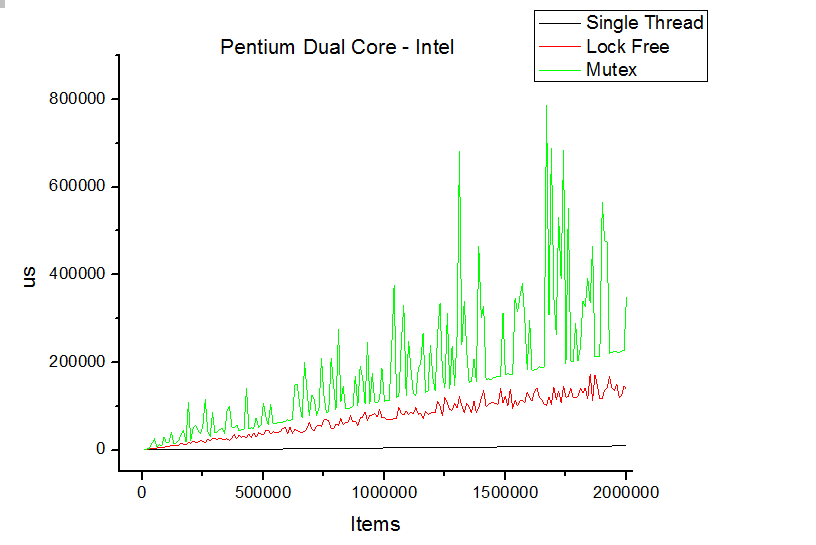
\includegraphics[width=120mm]{linux.png}
\caption{Computational time in milliseconds for enqueuing/dequeuing of 2,000,000 items on a Linux Server.}
\label{fig:linux}
\end{figure}

\begin{figure}[htp]
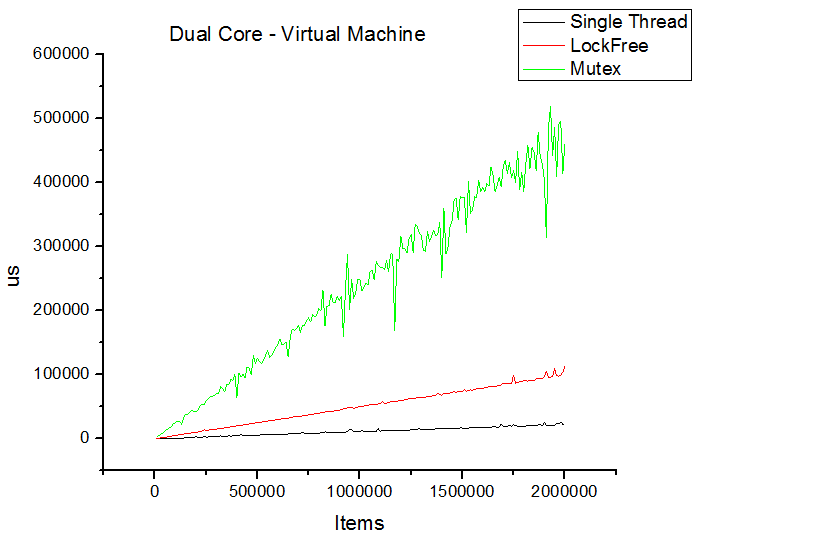
\includegraphics[width=120mm]{windows.png}
\caption{Computational time in milliseconds for enqueuing/dequeuing of 2,000,000 items on Windows 7.}
\label{fig:windows}
\end{figure}

We also run it within a Virtual Machine (VMWare) Running inside Windows 7 (SuSe Linux and Intel Pentium Dual-Core CPU). In figure \ref{fig:windows}, it can be seen that for 2,000,000 items each algorithm takes the following times in milliseconds to enqueue/dequeue all:	single-threaded, 24ms; lock-free: 114ms; mutex queue, 460ms.

It can be seen by these results that for both systems, Linux Server and Windows 7, the mutex queue provides the worst results in computational time when compared against the lock-free approach.

Also for both systems, it can be seen that the single-threaded approach provides much better results than the multi-threaded approaches, since these are not bound to any particular CPU and are subject to context switching and other factors.

\section{Conclusion}
\label{sec:conclusion}

As mentioned before, it is counterintuitive that the multi-threaded approach would be slower than the single-threaded approach, as we are dividing the work so we should theoretically finish the same ammount of work 2x faster. However, due to context switching, after all our threads are not bound to any particular CPU, cache hit/miss and other factors the multithreded version runs worse than its single thread counter part.

That being said, the intent of this paper was to show how mutexes are much slower compared to lock-free implementations for the same data structures. On the Virtual Machine we can see that the lock-free approach is very close to the single threaded one, while the mutex impacts the performance the most. Running outside the VM, on SuSe linux as well, we see that the mutex exhibits a behavior that is better than within the VM, but still worse than the lock-free implementation.

We can conclude then that lock-free has obvious advantages over their mutex counterparts but they don't come cheap. There are many factors to take in consideration when implementing lock-free data structures, particularly the ABA problem and other issues (cache line contention, context switching, live-locks and \textit{etc}.) that must be overcome so that one can take full advantage of this concurrency model.

In future work, different lock-free approaches will be compared, aiming to benchmark several non-blocking algorithms under certain criteria such as computational time.

\bibliographystyle{unsrt}
\bibliography{mybibliography}

%\bibliography{refs}
%\hyperref[Dr. Dobbs Lock Free Article]{''http://www.ddj.com/hpc-high-performance-computing/210604448''}
%\linebreak
%\hyperref[Herb Sutter's Website]{''http://herbsutter.com/2008/10/30/effective-concurrency-writing-a-generalized-concurrent-queue/''}
%\linebreak
%\hyperref[a]{''http://www.research.att.com/\textasciitilde bs/lock-free-vector.pdf''}
%\linebreak
%\hyperref[b]{''http://www.nwcpp.org/Downloads/2005/Lock-Free.pdf''}
%\linebreak
%\hyperref[c]{''http://erdani.org/publications/cuj-2004-12.pdf''}
%\linebreak
%\hyperref[d]{''http://erdani.org/publications/cuj-2004-10.pdf''}
%\linebreak
%\hyperref[e]{''http://softwarecommunity.intel.com/articles/eng/1664.htm''}
%\linebreak
%\hyperref[f]{''http://www.grame.fr/pub/LockFree.pdf''}
%\linebreak
%\hyperref[g]{''http://www.grame.fr/pub/TR-050523.pdf''}
%\linebreak
%\hyperref[h]{''http://www.lenholgate.com/archives/000492.html''}
%\linebreak
%\hyperref[i]{''http://www.ddj.com/cpp/189401457''}
%\linebreak
%\hyperref[j]{''http://tim.klingt.org/git?p=boost\_lockfree.git;a=summary''}
%\linebreak

\end{document}
